\subsection{\href{https://tensornetwork.org/mps/}{Matrix Product State / Tensor Train}}



Matrix Product State ($\textit{MPS}$) или $tensor \hspace{3mm} train$ ($\textit{TT}$) - это факторизация тензора с N индексами в цепочеч-ное произведение трехиндексных тензоров. Это частный случай tree tensor network ($\textit{TTN}$).



$\textit{TT}$ факторизация тензора $\textit{T}$ может быть представлена в графической нотации Пенроуза

\begin{figure}[h!tp]
\centering
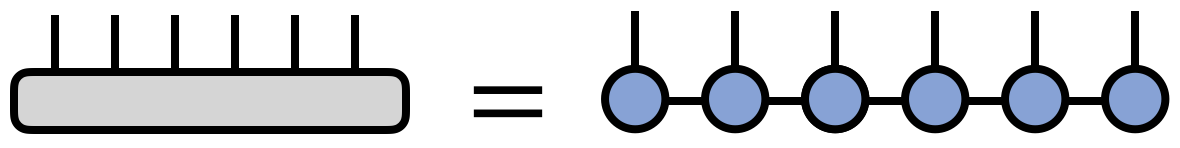
\includegraphics[scale=0.3]{MatrixProductState_TensorTrain/mpstt_diagram.png}
\caption{TT факторизация в нотации Пенроуза}
\label{fig:TTFactorizationDiag}
\end{figure}

В то же время, $\textit{TT}$ факторизация тензора $\textit{T}$ представима в традиционной нотации:

\begin{equation}
T^{s_1 s_2 s_3 s_4 s_5 s_6} = \sum_{\{\mathbf{\alpha}\}} A^{s_1}_{\alpha_1} 
A^{s_2}_{\alpha_1 \alpha_2}
A^{s_3}_{\alpha_2 \alpha_3} 
A^{s_4}_{\alpha_3 \alpha_4} 
A^{s_5}_{\alpha_4 \alpha_5} 
A^{s_6}_{\alpha_5}
\end{equation}

где $\alpha_i$ - это размерности тензоров A.



Важно понимать, что тензоры в тензорном поезде соединяются с помощью ребер, имеющие размерности $d_i$. К примеру, если есть тензор $T^{s_1 s_2 \cdots s_N}$, имеющий $N$ ребер с размерностями $d$, то тензор всегда может быть представлен в виде $\textit{TT}$ с размерностью $m = d^{\frac{N}{2}}$



К тому же тензор с $N$ ребрами с размерностями $d$
должен определяться $d^N$ параметрами, но представ-ление этого вектора с помощью $\textit{TT}$ с рангом $m$ требует $Ndm^2$ параметров. При этом, кол-во параметров можно еще сильнее уменьшить.



Извлечение тензора размерности 1 из тензора стоит $Nm^2$. Если есть тензор 

\begin{equation}
T^{s_1 s_2 s_3 \cdots s_N} = \sum_{\{\mathbf{\alpha}\}} 
A^{s_1}_{\alpha_1} 
A^{s_2}_{\alpha_1 \alpha_2}
A^{s_3}_{\alpha_2 \alpha_3} 
\cdots
A^{s_N}_{\alpha_{N-1}},
\end{equation}

то извлечь из него тензор размерности 1 можно следующим образом -- фиксируем $s_j$ для каждого $A$. Затем свернем тензоры $A^{s_1}_{\alpha_1}$ и $A^{s_2}_{\alpha_1 \alpha_2}$ по $\alpha_1$ и получим результирующий вектор $L_{\alpha_2}$, который затем свернется с $A^{(s_3)}_{\alpha_2 \alpha_3}$. Продолжая то же действие, мы получим $s_1,s_2,s_3,\ldots,s_N$ компонент через последова-тельность векторно-матричных умножений.\\

Что касается произведения двух $\textit{TT}$, то имея два тензора \begin{equation}
T^{s_1 s_2 s_3 s_4 s_5 s_6} = \sum_{\{\mathbf{\alpha}\}} 
A^{s_1}_{\alpha_1} 
A^{s_2}_{\alpha_1 \alpha_2}
A^{s_3}_{\alpha_2 \alpha_3} 
A^{s_4}_{\alpha_3 \alpha_4} 
A^{s_5}_{\alpha_4 \alpha_5} 
A^{s_6}_{\alpha_5}
\end{equation} и 
\begin{equation}
W^{s_1 s_2 s_3 s_4 s_5 s_6} = \sum_{\{\mathbf{\beta}\}} 
B^{s_1}_{\beta_1} 
B^{s_2}_{\beta_1 \beta_2}
B^{s_3}_{\beta_2 \beta_3} 
B^{s_4}_{\beta_3 \beta_4} 
B^{s_5}_{\beta_4 \beta_5} 
B^{s_6}_{\beta_5},
\end{equation} мы получим 
\begin{equation}
\langle T, W\rangle =
\sum_{\{\mathbf{s}\}} 
T^{s_1 s_2 s_3 s_4 s_5 s_6} 
W^{s_1 s_2 s_3 s_4 s_5 s_6} 
\end{equation}

Сложность такого алгоритма составит $Nm^3d$.



Особенно мощной операцией является сжатие тензорной сети в форму $\textit{TT}$. Для конкретики предполо-жим, что  мы хотим сжать TT размерности $M$  до размерности $m$, так чтобы новый $\textit{TT}$ был как можно ближе к исходному, в смысле евклидова расстояния. Процедура сжатия начинается со свертки двух копий входной сети $\textit{TT}$ по всем внешним индексам, кроме последнего внешнего индекса.
Чтобы эффективно вычислить свертку двух копий $\textit{TT}$, формируются промежуточные тензоры $E_1, E_2,...$  как показано на иллюстрации.

\begin{figure}[h!tp]
\centering
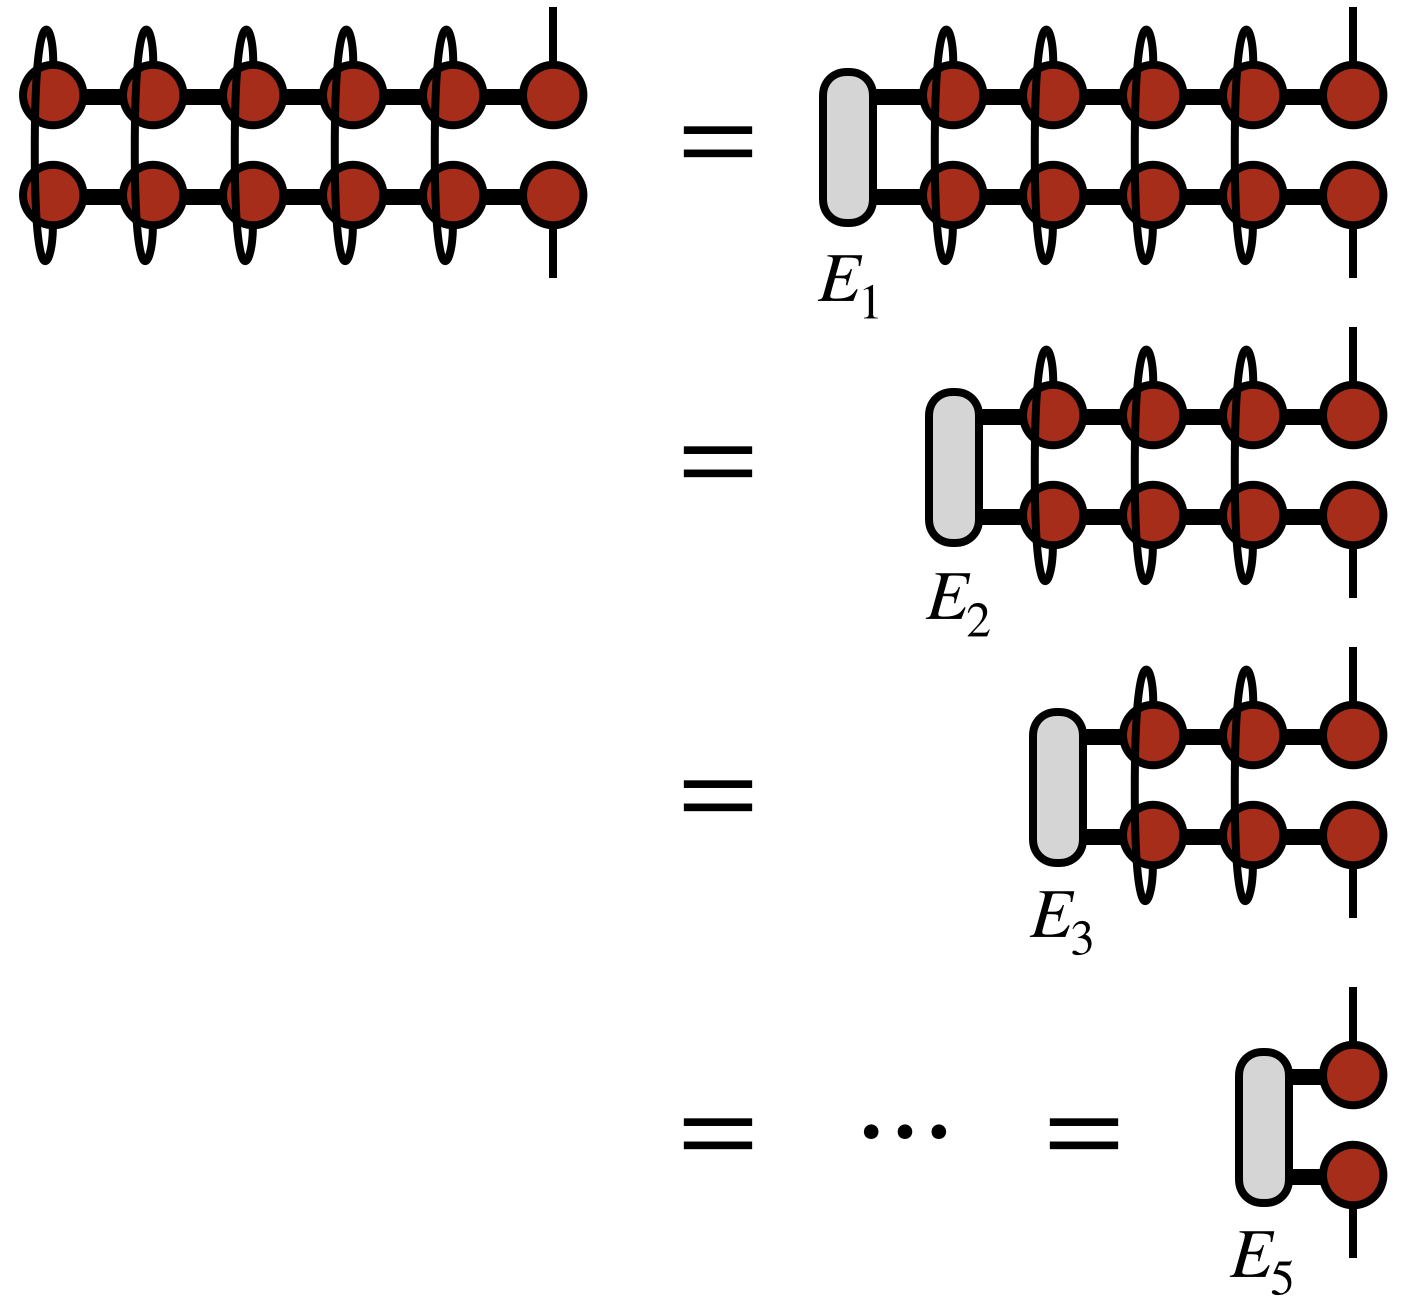
\includegraphics[scale=0.3]{MatrixProductState_TensorTrain/dm_comput.png}
\caption{Преобразование свертки копий}
\label{fig:ConvDiag1}
\end{figure}

Вычислив все $E_j$ можно сформировать $\rho_6$ reduced density matrix - квадрат тензора, представленного сетью, суммируемый по всем, кроме его последнего индекса.

\begin{figure}[h!tp]
\centering
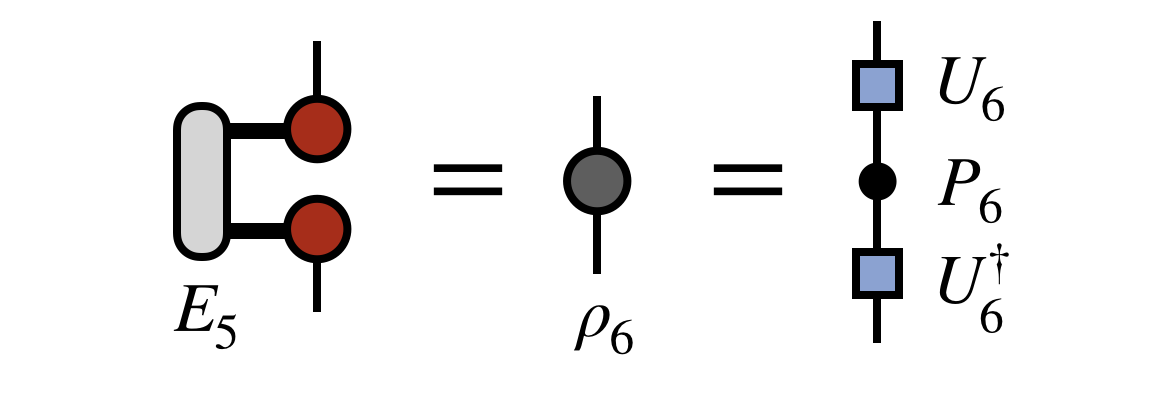
\includegraphics[scale=0.3]{MatrixProductState_TensorTrain/diag_rho6.png}
\caption{Reduced density matrix}
\label{fig:ReducedDensityMatrixDiag}
\end{figure}

Это эрмитова матрица, поэтому она всегда может быть диагонализирована унитарной $U_6$. 



Чтобы сформировать новый тензор из сжатого $\textit{TT}$, то мы формируем новую матрицу плотности и диагонализируем ее

\begin{figure}[h!tp]
\centering
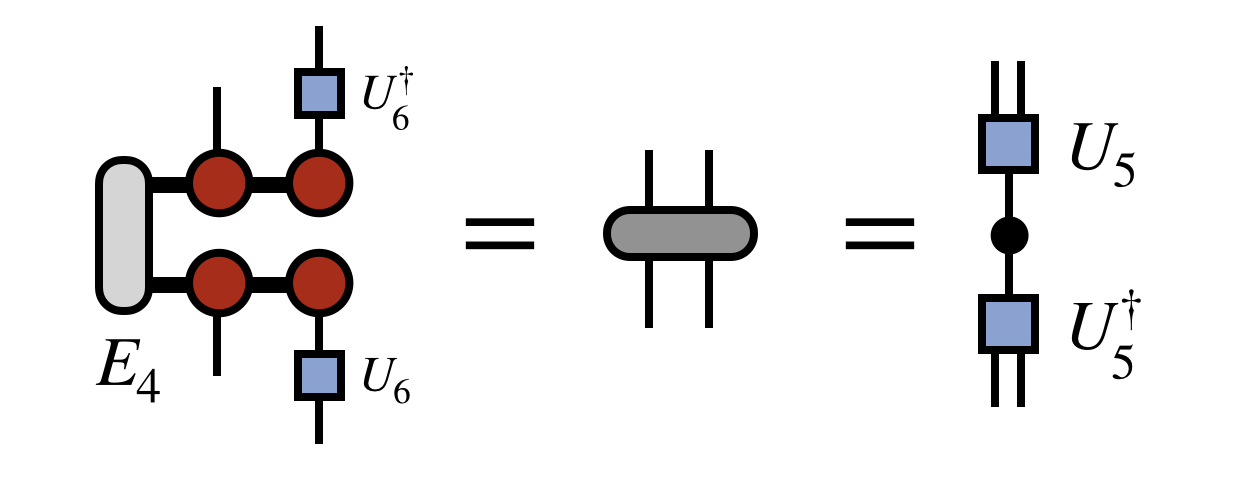
\includegraphics[scale=0.3]{MatrixProductState_TensorTrain/diag_rho56.png}
\caption{Следующий шаг}
\label{fig:NextStepDiag}
\end{figure}

\newpage

Получив $U_5$ как показано выше, вычисляется следующая матрица плотности, снова используя все предыдущие $U$ тензоры для поворота и сжатия пространства, охватываемого всеми предыдущими внеш-ними индексами

\begin{figure}[h!tp]
\centering
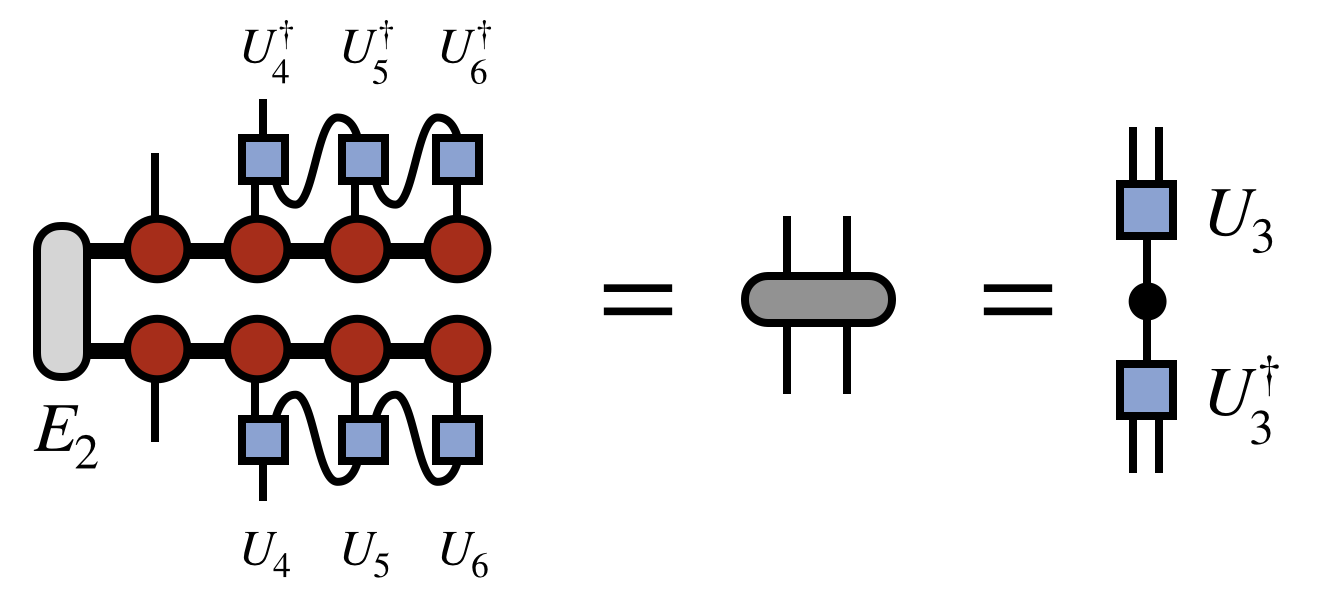
\includegraphics[scale=0.3]{MatrixProductState_TensorTrain/diag_rho3456.png}
\caption{Следующая итерация}
\label{fig:NextIterDiag}
\end{figure}

После того, как мы получаем все $U$ тензоры, повторяя шаги выше, получим первый тензор нового $\textit{TT}$ с помощью следующей сверточной диаграммы

\begin{figure}[h!tp]
\centering
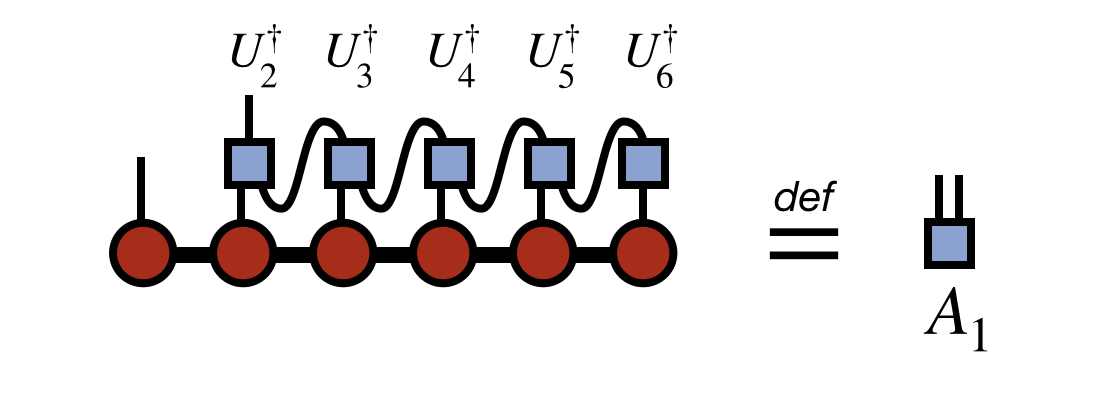
\includegraphics[scale=0.3]{MatrixProductState_TensorTrain/first_tensor.png}
\caption{Сверточная диаграмма}
\label{fig:ConvDiag}
\end{figure}

Так соединив $A_1$ со всеми $U_j$ получим новый сжатый тензор.

\begin{figure}[h!tp]
\centering

\includegraphics[scale=0.3]{MatrixProductState_TensorTrain/compressed_mpstt.png}
\caption{Сжатый тензор}
\label{fig:ComprTensorDiag}
\end{figure}